Για την άσκηση αυτή χρησιμοποιήθηκαν οι εξής βιβλιοθήκες:
\begin{itemize}
    \item \texttt{fast\_vdd1v2\_basicCells.lib} για τον χρονισμό
    \item \texttt{gsclib045\_macro.lef}, \texttt{gsclib045\_tech.lef} για τα φυσικά χαρακτηριστικά και
    \item \texttt{gpdk045.tch} για τα παράσιτα.
\end{itemize}

Παρατηρείται ότι δημιουργείται αυτόματα η λειτουργική συνθήκη "nominal" με τιμές PVT = (process 1.000000, voltage 1.320000 V, temperature $0^{\circ}C$), γεγονός που αντιστοιχεί σε γρήγορη γωνία λειτουργίας (fast corner).

Ο αναλυτής της βιβλιοθήκης αναφέρει ένα μήνυμα LBR-518, που δηλώνει ότι μία έξοδος κάποιου κυκλώματος δεν διαθέτει χαρακτηριστικό Boolean «function». Εμφανίζονται επίσης πολλαπλά προειδοποιητικά μηνύματα LBR-9 για τα κελιά ANTENNA και DECAP[2..10], τα οποία δεν έχουν καθορισμένες εξόδους. Το Genus επισημαίνει ότι τέτοια κελιά χαρακτηρίζονται ως "unusable timing models" και δεν χρησιμοποιούνται κατά τη διαδικασία αντιστοίχισης (mapping).

Στη συνέχεια, το εργαλείο ορίζει τη μεταβλητή \texttt{lef\_library} με δύο αρχεία: \texttt{gsclib045\_tech.lef} και \texttt{gsclib045\_macro.lef} (με αυτή τη σειρά). Κατά τη φόρτωσή τους, εμφανίζονται πολλά μηνύματα PHYS-129 τύπου "Via with no resistance", που δηλώνουν ότι για κάθε συγκεκριμένο via η τιμή αντίστασης ορίζεται αυτόματα σε 0.0 $\Omega$, εκτός αν δοθεί διαφορετικά.

Μετά την ανάγνωση, το Genus αναφέρει: «According to lef\_library, there are total 11 routing layers [V(5)/H(6)]», και επίσης: «Library has 324 usable logic and 128 usable sequential lib-cells».

Αμέσως μετά, εμφανίζεται μεγάλος αριθμός προειδοποιήσεων PHYS-279, που αναφέρουν ότι δεν βρέθηκαν φυσικοί ορισμοί (LEF) για πολλά κελιά, όπως DFF2RX1, DFF4X1, FILL1, FSWX1, HSWDX1 κ.ά. Το μήνυμα επαναλαμβάνεται έως το όριο των 20 εμφανίσεων (MESG-11). Το περιεχόμενο διευκρινίζει ότι τα συγκεκριμένα κελιά υπάρχουν λογικά στη βιβλιοθήκη χρονισμού αλλά δεν διαθέτουν φυσική περιγραφή (LEF).

Τέλος, φορτώνεται το αρχείο QRC (\texttt{gpdk045.tch}), όπου αναφέρεται: «According to qrc\_tech\_file, there are total 11 routing layers [V(5)/H(6)]», και η διαδικασία ολοκληρώνεται με το μήνυμα «Done reading qrc\_tech\_file». Η αναφορά του πλήθους των επιπέδων (11) είναι συνεπής μεταξύ LEF και QRC.

Στη συνέχεια το κύκλωμα αναλύεται (elaboration) και ελέγχεται (design check) χωρίς σφάλματα. Έπειτα δημιουργείται το αρχείο \texttt{constraints.sdc} με τους εξής περιορισμούς για τη σύνθεση που ορίζονται:

\begin{itemize}
    \item Ρολόι με 50\% duty cycle, συχνότητας 250 MHz και όνομα clk
    \item Καθυστέρηση (latency) του σήματος του ρολογιού στα 200 ps (0.2 ns)
    \item Αβεβαιότητα του σήματος ρολογιού στα 20 ps (0.02 ns)
    \item Χρόνος μετάβασης (ανόδου/καθόδου) του ρολογιού στο 1\% της περιόδου του (0.04 ns)
    \item Καθυστέρηση των εξόδων για όλες τις εξόδους του κυκλώματος για την ανάλυση χρονισμού setup στα 0.50 ns
    \item Καθυστέρηση των εξόδων για όλες τις εξόδους του κυκλώματος για την ανάλυση χρονισμού hold στα 0.25 ns
    \item Φορτίο όλων των εξόδων για ανάλυση χρονισμού setup στα 0.3 pF
    \item Φορτίο όλων των εξόδων για ανάλυση χρονισμού hold στα 0.04 pF
    \item Καθυστέρηση των εισόδων για όλες τις εισόδους του κυκλώματος για την ανάλυση χρονισμού setup στα 0.50 ns
    \item Καθυστέρηση των εισόδων για όλες τις εισόδους του κυκλώματος για την ανάλυση χρονισμού hold στα 0.25 ns
    \item Το κελί BUFX2 για την ανάλυση setup και το κελί BUFX8 για την ανάλυση hold.
\end{itemize}

Οι περιορισμοί φορτώνονται (\texttt{read\_sdc}) και ελέγχονται (\texttt{check\_timing\_intent}) χωρίς σφάλματα. Μετά τον ορισμό των μονοπατιών I2O, I2R, R2O και R2R εκτελούνται τα τρία βήματα της σύνθεσης (\texttt{syn\_generic}, \texttt{syn\_map}, \texttt{syn\_opt}).
Χρησιμοποιήθηκε η εντολή \texttt{set\_db / .use\_scan\_seqs\_for\_non\_dft false} για να αποτραπεί η αντικατάσταση των κανονικών DFFs με SDFFS.

Για τα αποτελέσματα παρατίθενται οι παρακάτω πίνακες όπως ζητείται στην εκφώνηση της εργασίας.

\begin{table}[H]
    \centering
    \caption{Total number of cells of each type}
    \begin{tabular}{lrrr}
        \toprule
        Type & Instances & Area ($\mu m^2$) & Area \% \\
        \midrule
        Sequential & 2399 & 18048.366 & 52.8 \\
        Inverter & 238 & 165.870 & 0.5 \\
        Buffer & 27 & 97.470 & 0.3 \\
        Logic & 6994 & 15865.722 & 46.4 \\
        \midrule
        \textbf{Total} & \textbf{9658} & \textbf{34177.428} & \textbf{100.0} \\
        \bottomrule
    \end{tabular}
\end{table}

Όπως φαίνεται στον Πίνακα 1.1, το συνολικό εμβαδόν των κελιών είναι περίπου $4177.428~\mu m^2$. Το εργαλείο εκτιμά εμβαδόν διασυνδέσεων (net area) $13902.342~\mu m^2$, καταλήγοντας σε συνολική επιφάνεια $48079.770~\mu m^2$.

\begin{table}[H]
    \centering
    \caption{Power consumption per category}
    \begin{tabular}{lrrrrr}
        \toprule
        Category & Leakage (mW) & Internal (mW) & Switching (mW) & Total (mW) & Row \% \\
        \midrule
        Memory & 0.0 & 0.0 & 0.0 & 0.0 & 0.0\% \\
        Register & $2.06\times10^{-3}$ & 4.04 & 3.21 & 7.26 & 66.30\% \\
        Latch & 0.0 & 0.0 & 0.0 & 0.0 & 0.0\% \\
        Logic & $2.20\times10^{-3}$ & 1.10 & 2.31 & 3.40 & 33.70\% \\
        Bbox & 0.0 & 0.0 & 0.0 & 0.0 & 0.0\% \\
        Clock & 0.0 & 0.0 & 0.0 & 0.0 & 0.0\% \\
        Pad & 0.0 & 0.0 & 0.0 & 0.0 & 0.0\% \\
        Pm & 0.0 & 0.0 & 0.0 & 0.0 & 0.0\% \\
        \midrule
        \textbf{Subtotal} & $4.26\times10^{-3}$ & 5.14 & 10.07 & 5.52 & 100.0\% \\
        \textbf{Percentage} & 0.04\% & 48.21\% & 51.75\% & 100.0\% & \\
        \bottomrule
    \end{tabular}
\end{table}

Όπως φαίνεται στον Πίνακα 1.2, η συνολική ισχύς του κυκλώματος είναι 10.7 mW.

\begin{table}[H]
    \centering
    \caption{Setup Slack for each path type}
    \begin{tabular}{lr}
        \toprule
        Category & Setup Slack (ns) \\
        \midrule
        I2O & - \\
        I2R & 2.141 \\
        R2O & 3.125 \\
        R2R & 0.994 \\
        \bottomrule
    \end{tabular}
\end{table}

Το εργαλείο δεν κατάφερε να βρει μονοπάτια του είδους I2O για να υπολογίσει το slack για αυτά. Αυτό σημαίνει ότι η σχεδίαση δεν περιέχει συνδυαστικά input $\rightarrow$ output μονοπάτια.

Έπειτα της εξαγωγής των αρχείων από το Genus για το Innovus, δημιουργήθηκε στο τελευταίο ένα design. Στη χωροθέτηση επιλέχθηκε το μέγεθος του die με διαστάσεις $250\times250~\mu m$. Παρατηρείται ότι το Core Utilization έχει τιμή 53\%. Μόλις προστεθεί χώρος 20 $\mu m$ μέχρι τα I/O, το Core Utilization έχει πλέον τιμή 75\%. Αυτό είναι αναμενόμενο και λογικό διότι το κενό δημιουργείται γύρω από το core για να εξασφαλίσει την ύπαρξη των δακτυλίων τροφοδοσίας, δεσμεύοντας ένα περιμετρικό τμήμα της διάταξης το οποίο δεν μπορεί πλέον να χρησιμοποιηθεί για την τοποθέτηση κελιών. Από τη στιγμή που το εμβαδόν των υπαρχόντων κελιών παραμένει αμετάβλητο και η διαθέσιμη επιφάνεια για την τοποθέτηση τους μικραίνει, το ποσοστό κάλυψης του core από κελιά, δηλαδή το utilization, αυξάνεται.

Έχοντας δημιουργήσει αυτό το κενό, τοποθετούνται οι δακτύλιοι με πάχος 4 $\mu m$, κενό διάστημα ανάμεσα τους 4 $\mu m$, κεντραρισμένοι στο διάκενο και χρησιμοποιώντας τα μέταλλα M10 και M11 της τεχνολογίας. Έπειτα, τοποθετούνται τρία σετ γραμμών με ίδιο πάχος και κενό. Χρησιμοποιήθηκε το μέταλλο M8 για τις οριζόντιες γραμμές και το M9 για τις κάθετες. Τέλος, τοποθετούνται οι ακροδέκτες τροφοδοσίας και γείωσης στο μέταλλο 10 στο μέσο της αριστερής γραμμής του εκάστοτε δακτυλίου και δημιουργούνται τα follow pins μέσω της εντολής \texttt{sroute}. Χρησιμοποιούνται όλα τα μέταλλα με ενεργοποιημένες τις επιλογές Allow Jogging και Allow Layer Change όπως συνίσταται.

\begin{figure}[H]
    \centering
    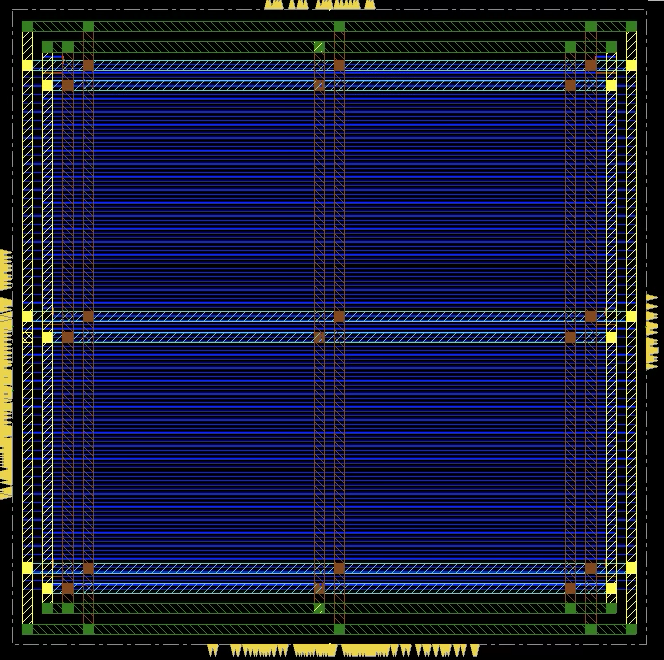
\includegraphics[width=0.8\textwidth]{assets/fig1_1_pdn.png}
    \caption{Power Distribution Network}
\end{figure}

Επόμενο βήμα είναι η τοποθέτηση. Επιλέγεται high effort για τον χρονισμό, καμία βελτιστοποίηση ισχύος και τοποθέτηση των I/O. Όλες οι υπόλοιπες παράμετροι αφήνονται όπως είναι. Παρακάτω ακολουθούν οι πίνακες με τα αποτελέσματα που ζητούνται. Η συνολική επιφάνεια είναι $34284.474~\mu m^2$.

\begin{table}[H]
    \centering
    \caption{Setup Slack for each path type pre Clock Tree Synthesis}
    \begin{tabular}{lr}
        \toprule
        Category & Setup Slack (ns) \\
        \midrule
        I2O & - \\
        I2R & 2.566 \\
        R2O & 3.053 \\
        R2R & 1.444 \\
        \bottomrule
    \end{tabular}
\end{table}

\begin{figure}[H]
    \centering
    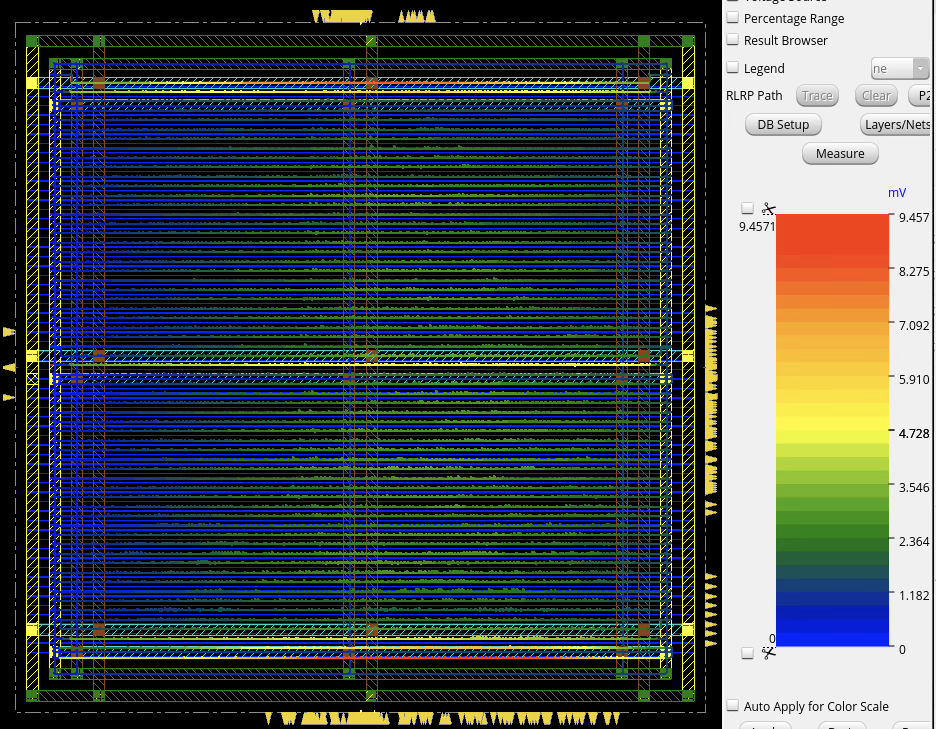
\includegraphics[width=0.8\textwidth]{assets/fig1_2_rail_analysis.png}
    \caption{Results of Early Power Rail Analysis}
\end{figure}

\begin{table}[H]
    \centering
    \caption{Power Consumption per Category pre Clock Tree Synthesis}
    \begin{tabular}{lrrrrr}
        \toprule
        Category & Leakage (mW) & Internal (mW) & Switching (mW) & Total (mW) & Row \% \\
        \midrule
        Sequential & $1.94\times10^{-3}$ & 3.556 & 0.521 & 4.079 & 43.65 \\
        Macro & 0.0 & 0.0 & 0.0 & 0.0 & 0.0 \\
        IO & 0.0 & 0.0 & 0.0 & 0.0 & 0.0 \\
        Combinational & $2.36\times10^{-3}$ & 1.486 & 3.779 & 5.267 & 59.35 \\
        Clock (Comb) & 0.0 & 0.0 & 0.0 & 0.0 & 0.0 \\
        Clock (Seq) & 0.0 & 0.0 & 0.0 & 0.0 & 0.0 \\
        \midrule
        \textbf{Total} & $4.27\times10^{-3}$ & \textbf{5.042} & \textbf{4.3} & \textbf{9.346} & \textbf{100.0} \\
        \bottomrule
    \end{tabular}
\end{table}

Στη συνέχεια γίνεται Early Power Rail ανάλυση. Ακολουθείται η διαδικασία που δίνεται στο εγχειρίδιο εργαστηρίου και προκύπτουν τα παρακάτω αποτελέσματα.

Φαίνεται από το οπτικοποιημένο αποτέλεσμα της ανάλυσης (Figure 1.2) ότι πολλές γραμμές εμφανίζουν πτώση τάσης. Θεωρώ αποδεκτή έως και 7\%, αν και όχι ιδανική. Η μεγαλύτερη πτώση τάσης εμφανίζεται στα rails της άνω και κάτω πλευράς, ρίχνοντας την τάση κατά 9.5 mV. Η τιμή αυτή αντιπροσωπεύει $\frac{9.5}{1320}\approx7.2\%$, ποσοστό οριακά ανεκτό στη συγκεκριμένη υλοποίηση, έτσι ώστε να θεωρείται ότι δεν επηρεάζει την λειτουργία του κυκλώματος. Πιθανότατα, σε εμπορική υλοποίηση να μην είναι αποδεκτό τέτοιο ποσοστό.

Η γραμμή τροφοδοσίας περνάει ακριβώς πάνω από τις περιοχές όπου εμφανίζεται η μεγαλύτερη πτώση τάσης. Αυτό μπορεί να σημαίνει ότι το κύκλωμα είναι πιο “λογικά πυκνό" σε εκείνο το μέρος (Figure 1.3) ή ότι η αντίσταση του grid είναι μεγαλύτερη.

\begin{figure}[H]
    \centering
    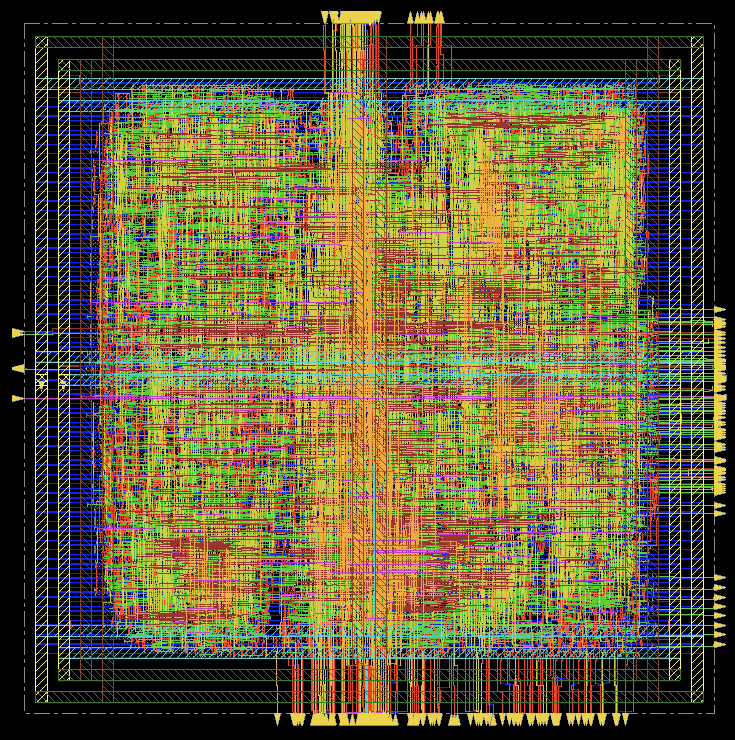
\includegraphics[width=0.8\textwidth]{assets/fig1_3_placement.png}
    \caption{Design Placement}
\end{figure}

Επόμενο στάδιο αποτελεί η Early Global Routing. Στην πρώτη περίπτωση καλύπτονται όλα τα μέταλλα στο εύρος δρομολόγησης (M1-M11) ενώ στη δεύτερη μόνο τα M5-M10. Εκτελώντας την εντολή \texttt{reportCongestion -hotspot} δεν παρατηρείται κάποια διαφοροποίηση: σε καμία περίπτωση δεν ανιχνεύεται συμφόρηση ή hotspot. Παρακάτω παρατίθενται οι πόροι που χρησιμοποιούνται σε καθεμία από τις περιπτώσεις.

\begin{table}[H]
    \centering
    \caption{Resources used for Early Global Routing}
    \begin{tabular}{lrr}
        \toprule
        Metals Used & Wirelength ($\mu m$) & Via (\#) \\
        \midrule
        M1-M11 & 202415.800 & 108727 \\
        M5-M11 & 202180.095 & 229240 \\
        \bottomrule
    \end{tabular}
\end{table}

Παρατηρείται ότι το μήκος των καλωδίων είναι παρόμοιο και στις δυο περιπτώσεις. Ωστόσο, κοιτάζοντας τα στατιστικά είναι εμφανές ότι η πλειοψηφία των καλωδίων θέλει να είναι σε όσο χαμηλότερο επίπεδο γίνεται. Μάλιστα, στην περίπτωση χρήσης των μετάλων M1-M11 τα μήκη στα επίπεδα M6-M11 είναι αμελητέα ενώ στην περίπτωση χρήσης των M5-M10 το ίδιο συμβαίνει στα επίπεδα M9-M10 (<10\%).

Όσον αφορά τα vias, είναι προφανής η διαφορά στο πλήθος που χρησιμοποιούνται. Παρότι το γεγονός ότι η δρομολόγηση των σημάτων περιορίστηκε στα μέταλλα M5-M10 η χρήση via1-via4 παραμένει σημαντική επειδή τα pins των κελιών εξακολουθούν να βρίσκονται στα μέταλλα M1/M2. Ο δρομολογητής πρέπει να δημιουργήσει via stacks για να φτάσει το M5, έχοντας ως αποτέλεσμα πολλαπλά vias χαμηλού επιπέδου χωρίς αντίστοιχο μήκος καλωδίου σε εκείνες τις στρώσεις. Αυτό εξηγεί την $2\times$ κατανάλωση πόρων vias παρά τη μηδενική οριζόντια δρομολόγηση στα χαμηλότερα μέταλλα.

Το επόμενο βήμα αφορά τη σύνθεση του δέντρου ρολογιού. Δημιουργείται ένα NDR με διπλάσιο πάχος και default κενό για όλα τα μέταλλα για το trunk του δέντρου και ο default NDR για τα leaves. Το ελάχιστο και μέγιστο επίπεδο είναι M6 και M7 αντίστοιχα, εφόσον το δίκτυο διανομής χρησιμοποιεί τα μέταλλα M11 έως M8. Τέλος, προστίθεται προστασία και από τις δύο μεριές στο ρολόι χρησιμοποιώντας το VSS net ως shield net, τίθεται 1 ns στρέβλωση και μέγιστος ρυθμός μετάβασης 0.04 ns. Από τη σύνθεση του δέντρου ρολογιού και τη βελτιστοποίηση του κυκλώματος προκύπτουν οι παρακάτω πίνακες.

Η σύνθεση χρησιμοποιεί 24 buffers ρολογιού και κανέναν αντιστροφέα. Στη σχεδίαση υπάρχει μοναδικό skew group. Η στρέβλωση που επιτεύχθηκε είναι 0.012 ns, πολύ μικρότερη από την επιθυμητή ενώ ο επιθυμητός μέγιστος ρυθμός μετάβασης ρολογιού δεν ξεπεράστηκε κατά 0.001 ns (worst transition $= 0.039ns$).

Το μέγιστο και ελάχιστο βάθος του δέντρου ρολογιού ήταν 1, γεγονός που σημαίνει ότι το δέντρο είναι "ρηχό" και κάθε καταχωρητής οδηγείται από ακριβώς έναν buffer (μέσω ενός επιπέδου διανομής). Ένα τόσο ρηχό δέντρο είναι ασυνήθιστο, ωστόσο κρίνεται αποδεκτό στη συγκεκριμένη περίπτωση λόγω του μικρού μεγέθους της σχεδίασης $(250\mu m \times 250\mu m)$, όπου η οδήγηση του σήματος μπορεί να επιτευχθεί αποτελεσματικά χωρίς πολλαπλά επίπεδα επαναληπτών. Το εργαλείο επέλεξε αυτή τη λύση ως τη βέλτιστη για την ικανοποίηση των χρονικών περιορισμών με ελάχιστη χρήση πόρων. Τέλος, το trunk έχει συνολικό μήκος διαδρομής 629.405 $\mu m$ και τα leaves $9072.510~\mu m$.

Ακολουθούν πίνακες με τα αποτελέσματα για setup και hold slack και την κατανάλωση ισχύος. Η συνολική επιφάνεια είναι $34627.842~\mu m^2$.

\begin{table}[H]
    \centering
    \caption{Setup and Hold Slack post Clock Tree Synthesis}
    \begin{tabular}{lrr}
        \toprule
        Category & Setup Slack (ns) & Hold Slack (ns) \\
        \midrule
        I2O & - & - \\
        I2R & 2.519 & 0.240 \\
        R2O & 3.052 & 0.296 \\
        R2R & 1.413 & 0.033 \\
        \bottomrule
    \end{tabular}
\end{table}

\begin{table}[H]
    \centering
    \caption{Power Consumption per Category post Clock Tree Synthesis}
    \begin{tabular}{lrrrrr}
        \toprule
        Category & Leakage (mW) & Internal (mW) & Switching (mW) & Total (mW) & Row \% \\
        \midrule
        Sequential & $1.93\times10^{-3}$ & 3.535 & 0.46 & 3.997 & 38.14 \\
        Macro & 0.0 & 0.0 & 0.0 & 0.0 & 0.0 \\
        IO & 0.0 & 0.0 & 0.0 & 0.0 & 0.0 \\
        Combinational & $2.38\times10^{-3}$ & 1.515 & 3.899 & 5.416 & 51.68 \\
        Clock (Comb) & $4.81\times10^{-5}$ & 0.232 & 0.8352 & 1.067 & 10.19 \\
        Clock (Seq) & 0.0 & 0.0 & 0.0 & 0.0 & 0.0 \\
        \midrule
        \textbf{Total} & $4.36\times10^{-3}$ & \textbf{5.283} & \textbf{5.194} & \textbf{10.48} & \textbf{100.0} \\
        \bottomrule
    \end{tabular}
\end{table}

Έπειτα ακολουθεί η δρομολόγηση. Επιλέγονται οι ρυθμίσεις Fix Antenna, SI Driven, Timing Driven με effort 5, Via Optimization με medium effort όπως ορίζει η εκφώνηση και παρακάτω βρίσκονται τα αποτελέσματα.
Ακολουθούν πίνακες με τα αποτελέσματα για setup και hold slack και την κατανάλωση ισχύος. Η συνολική επιφάνεια είναι $34627.842~\mu m^2$.

\begin{table}[H]
    \centering
    \caption{Setup and Hold Slack post Routing}
    \begin{tabular}{lrr}
        \toprule
        Category & Setup Slack (ns) & Hold Slack (ns) \\
        \midrule
        I2O & - & - \\
        I2R & 2.531 & 0.241 \\
        R2O & 3.054 & 0.295 \\
        R2R & 1.452 & 0.032 \\
        \bottomrule
    \end{tabular}
\end{table}

\begin{table}[H]
    \centering
    \caption{Power Consumption per Category post Routing}
    \begin{tabular}{lrrrrr}
        \toprule
        Category & Leakage (mW) & Internal (mW) & Switching (mW) & Total (mW) & Row \% \\
        \midrule
        Sequential & $1.93\times10^{-3}$ & 3.537 & 0.452 & 3.991 & 38.15 \\
        Macro & 0.0 & 0.0 & 0.0 & 0.0 & 0.0 \\
        IO & 0.0 & 0.0 & 0.0 & 0.0 & 0.0 \\
        Combinational & $2.38\times10^{-3}$ & 1.513 & 3.863 & 5.379 & 51.43 \\
        Clock (Comb) & $4.81\times10^{-5}$ & 0.232 & 0.858 & 1.09 & 10.42 \\
        Clock (Seq) & 0.0 & 0.0 & 0.0 & 0.0 & 0.0 \\
        \midrule
        \textbf{Total} & $4.355\times10^{-3}$ & \textbf{5.283} & \textbf{5.173} & \textbf{10.46} & \textbf{100} \\
        \bottomrule
    \end{tabular}
\end{table}

Τέλος, ελέγχεται το φυσικό σχέδιο για DRC παραβιάσεις μέσω της εντολής \texttt{verify drc}. Στη συνέχεια προστίθενται Fillers σε όλα τα επίπεδα με ελάχιστο όριο πυκνότητας το 10\% για όλα τα μέταλλα.

Εμφανίστηκαν DRC παραβάσεις οι οποίες δεν λύθηκαν με την εκτέλεση της εντολής \texttt{ecoroute -fix\_drc} και παρατίθενται παρακάτω.
\begin{itemize}
    \item Metal Short
    \item Metal Spacing
    \item End-of-Line Spacing
\end{itemize}